\begin{frame}{Meter imágenes es sencillo\ldots{}}
    \begin{block}{\textbackslash \texttt{includegraphics[ops]\{img-path\}}}
    Mandato para incluir una imagen en el documento, siguiendo las opciones especificadas...
    
    \begin{itemize}
        \item \textbf{Opciones de una imagen} (ops)
        \begin{itemize}
            \item \texttt{scale}
            \item \texttt{width}
            \item \texttt{height}
            \item \texttt{angle}
        \end{itemize}
    \end{itemize}        
    
    \end{block}    

\end{frame}

\begin{frame}[fragile]{Meter imágenes es sencillo no?\ldots{} no?}

{\small
    \begin{minted}{latex}
        \graphicspath{ {images/} }
        ...
        \includegraphics[width=5cm]{frog.jpeg}
    \end{minted}
}
    \vspace{1cm}
    \pause
    \begin{center}
        \includegraphics[width=5cm]{images/frog.jpeg}
    \end{center}
\end{frame}


\begin{frame}[fragile]{Meter imágenes es sencillo no?\ldots{} no?}
    \begin{block}{\texttt{\textbackslash begin\{figure\}[ops]\ldots{} \textbackslash end\{figure\}}}
    Bloque que permite insertar una imagen con mayor control sobre el posicionamiento, así como añadir más información (captions y ref).    
    \end{block}
    \textbf{Opciones de posicionamiento} (se pueden combinar)
    \begin{itemize}
        \item \texttt{h}: donde el código (``here'')
        \item \texttt{t}: al inico de la página (``top'')
        \item \texttt{b}: al final de la página (``bottom'')
        \item \texttt{p}: en una nueva página (``page'')
        \item \texttt{!}: fuerza la posicion dada
        \item \texttt{H}: requiere pkg. \texttt{float}
    \end{itemize}
    
\end{frame}


\begin{frame}[fragile]{Meter imágenes es sencillo no?\ldots{} no?}

    {\small
    \begin{minted}{latex}
    \begin{figure}%[ h t b p ! H ]
        \centering
        \includegraphics[width=5cm]{frogs.jpeg}
        \caption{Frongus}
        \label{fig:frongus}
    \end{figure}
    \end{minted}
    }

    \pause
    
    \begin{figure}
        \centering
        \includegraphics[width=5cm]{images/frogs.jpeg}
        \caption{Frongus}
        \label{fig:frongus}
    \end{figure}
\end{frame}


\begin{frame}{Meter imágenes \textbf{bien} no es sencillo...}{Alrededor de texto (\texttt{wrapfig})}

    \pause
    % Del paquete (como no) wrapfig
    \begin{wrapfigure}{r}{0.5\textwidth}
        \begin{figure}
            \centering
            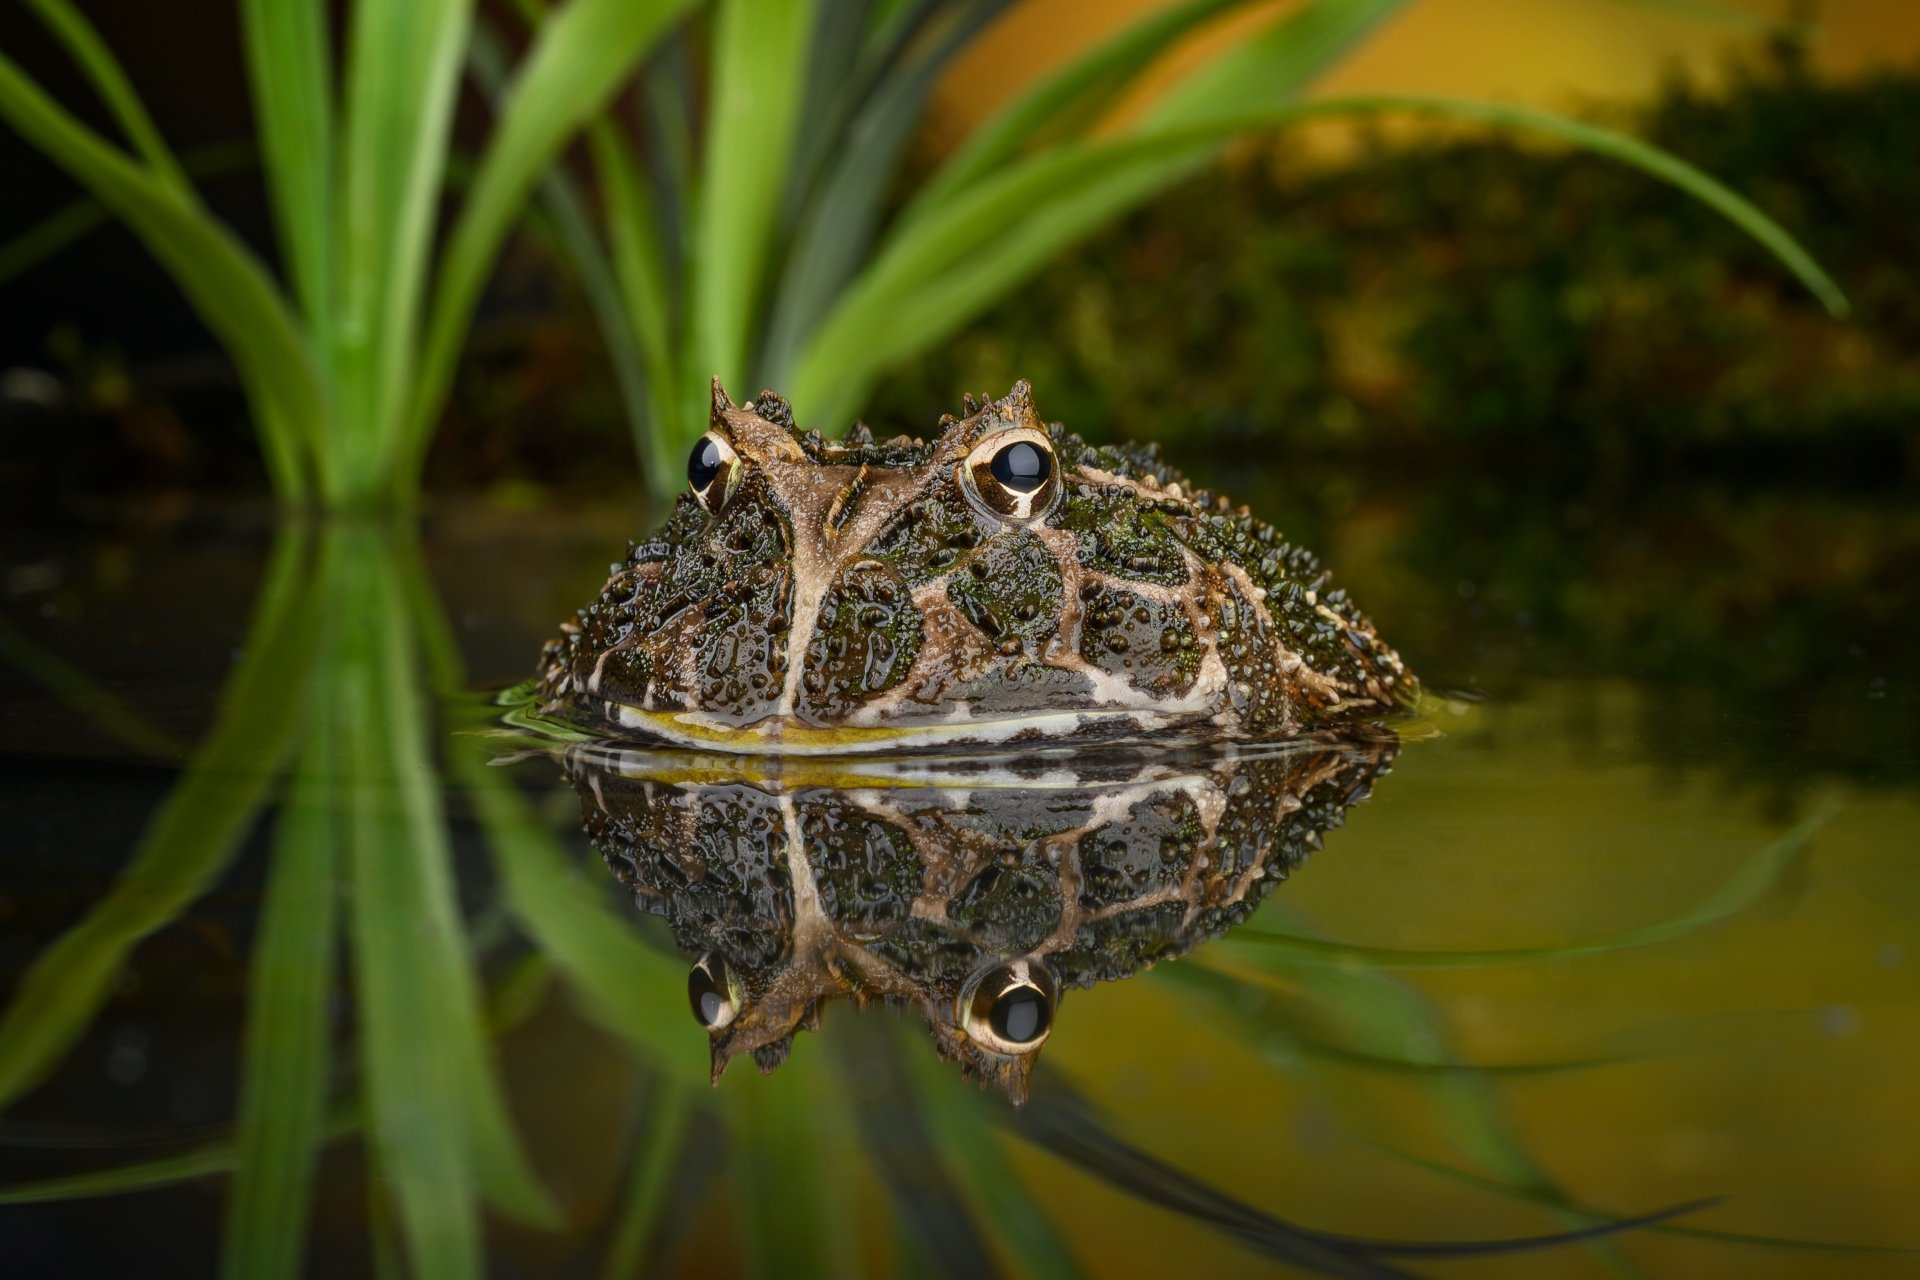
\includegraphics[width=5cm]{images/le_frog.jpeg}
            \caption{Le Frog}
            \label{fig:le_frog}
        \end{figure}
    \end{wrapfigure}
    Texto que habla de la Figura \ref{fig:le_frog}\ldots{}
    \blindtext
    
\end{frame}

\begin{frame}[fragile]{Meter imágenes \textbf{bien} NO es sencillo...}{Alrededor de texto (\texttt{wrapfig})}

{\small
\begin{minted}{latex}
    Texto...
    % r es right, pero
    % % r-R | l-L | i-I | o-O (mayus = float)
    \begin{wrapfigure}{r}{0.5\textwidth}
        \begin{figure}
            \centering
            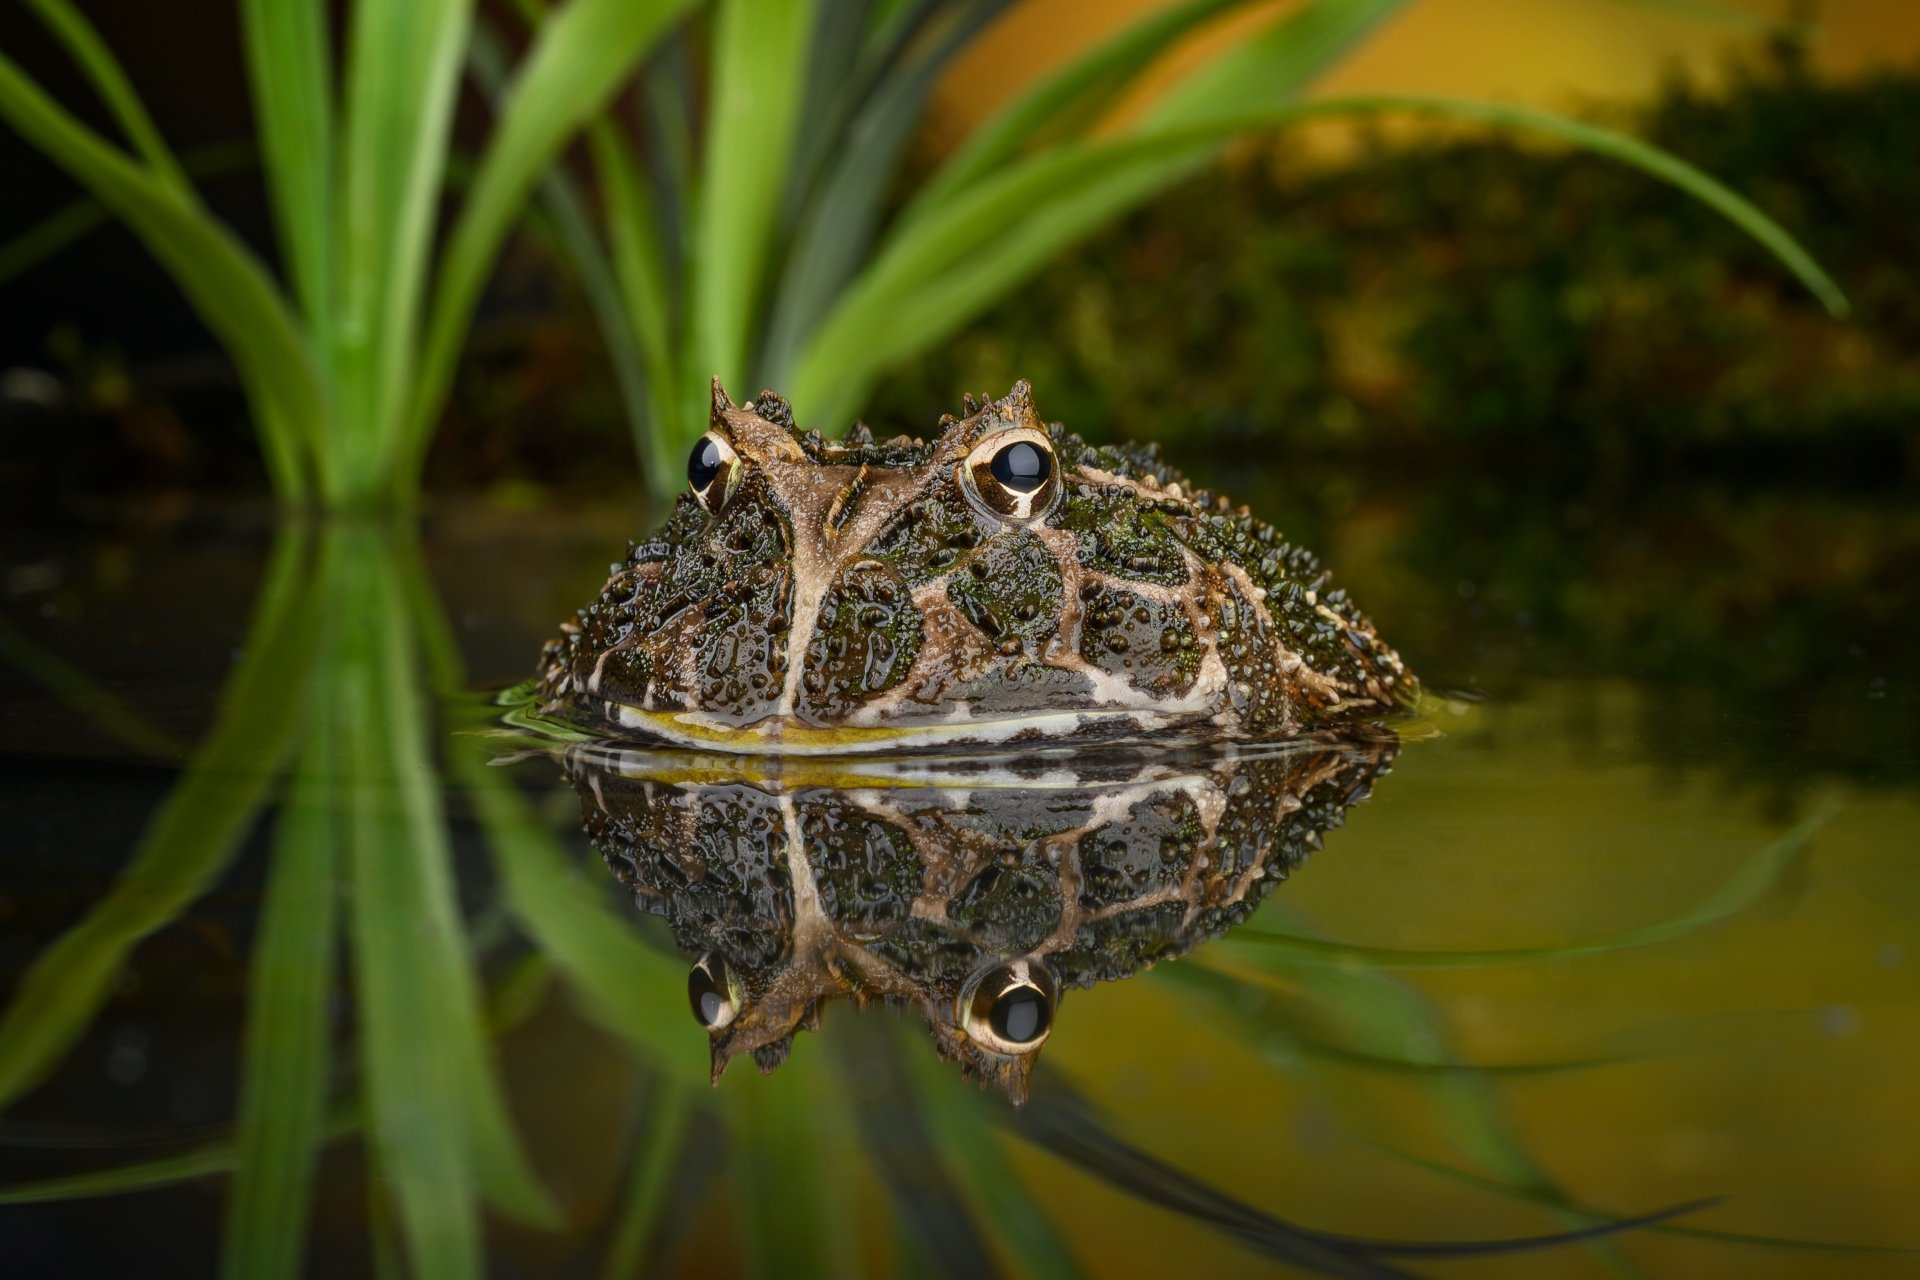
\includegraphics[width=5cm]{images/le_frog.jpeg}
            \caption{Le Frog}
            \label{fig:le_frog} % Genera ref para \ref
        \end{figure}
    \end{wrapfigure}
    Texto que habla de la Figura \ref{fig:le_frog}\ldots{}
    Más texto...
\end{minted}
}
    
\end{frame}

